\documentclass{article}

\usepackage[margin=1in]{geometry}
\usepackage[utf8]{inputenc}
\usepackage[english]{babel}
\usepackage[linktoc=all]{hyperref}
\usepackage{indentfirst}
\usepackage{titlesec}
\usepackage{tocloft}
\usepackage{setspace}
\usepackage{enumitem}
\usepackage{float}
\usepackage{fancyhdr}
\usepackage{lmodern}
\usepackage{tabularx}
\usepackage{array}
\usepackage{parallel}
\usepackage{lipsum}
\usepackage{graphicx}
\usepackage[dvipsnames, table]{xcolor}
\renewcommand{\cftsecleader}{\cftdotfill{\cftdotsep}}
\newcommand\sectionbreak{\clearpage}
\usepackage{placeins}

\title{\textbf{Human-Computer Interaction} \\ \Large{CS 420/620} \\ \large{Project Part 3: Design} \vspace{+16ex}}

\author{\textbf{\Large Team 01: PyBank} \\ \large{Brianna Blain-Castelli and Nikkolas Irwin}}
\date{\vspace{-2ex} \large{November 15, 2019}}


\begin{document}

\maketitle

\begin{center}
    \vspace{+16ex}
    {\textbf{\Large{Department of Computer Science and Engineering}} \\
    \large{College of Engineering, University of Nevada, Reno} \\
    \large{Course Instructor: Dr. Sergiu Dascalu}}
\end{center}

\pagenumbering{gobble}
\newpage

\pagenumbering{roman}
\tableofcontents

\newpage
\setlength{\cftfigindent}{0pt}  % remove indentation from figures in lof
% \setlength{\cfttabindent}{0pt}  % remove indentation from tables in lot
\listoffigures
% \listoftables

\newpage

\doublespacing
\pagenumbering{arabic}
%-----------------------------------START-----OF-----SECTION--------------------------------%
\section{Abstract}
\label{sect:abstract}

PyBank, an interactive Python GUI application, simulates a desktop client for personal banking. The application will contain a number of common banking processes such as creating an a new banking account, checking account information, depositing funds, withdrawing funds, and some analytical analysis related to an accounts spending over time. The goal of this application, beyond simulating common banking processes, is to implement principles of human-computer interaction such as the Fundamental Principles of Interaction~\cite{THE_DESIGN_OF_EVERYDAY_THINGS:1} and the Eight Golden Rules of Interface Design~\cite{DESIGNING_THE_USER_INTERFACE:2} so that the application provides an enjoyable experience to its end-users. 

% EOF
%-----------------------------------END-----OF-----SECTION----------------------------------%
\newpage
%-----------------------------------START-----OF-----SECTION--------------------------------%
\section{High Level Design}
\label{sect:high_level_design}

Included below in the following sub-sections (Section~\ref{sect:architectural_diagram}~and Section~\ref{sect:activity_diagram}) are an architectural diagram and activity diagram which describe some high-level design features of PyBank.

\subsection{System-Level Structural Diagram}
\label{sect:architectural_diagram}

The high-level components of PyBank can be listed broadly as the following:
\begin{itemize}
    \item {PyBank PyQt5 GUI}
    \item {Navigation Menu Component}
    \item {Login Component}
    \item {Sign-up Component}
    \item {Account Overview Component}
    \item {Checking Account Component}
        \begin{itemize}
            \item {Show Graphs Component}
            \item {Deposit Component}
            \item {Withdraw Component}
        \end{itemize}
    \item {Savings Account Component}
        \begin{itemize}
            \item {Show Graphs Component}
            \item {Deposit Component}
            \item {Withdraw Component}
        \end{itemize}
    \item {Credit Card Account Component}
        \begin{itemize}
            \item {Show Graphs Component}
            \item {Make A Payment Component}
            \item {Request Credit Line Increase Component}
        \end{itemize}
    \item {CSV File I/O Component}
\end{itemize}

The relationship between the PyBank PyQt5 GUI application and it's related components are further depicted in the architectural diagram shown below in Figure~\ref{fig:architectural_diagram}. This figure shows the components that are enclosed within the PyBank PyQt5 GUI as well as the CSV File I/O component which handles transaction processing for each PyBank customer. Unidirectional arrows convey an association between one component and another. For example, the Navigation Menu component is associated with six other components in the application. Bidirectional arrows convey both association and communication between two components in the application. Finally, dotted arrows are drawn to make it easier to visualize arrows that must cross the boundary of another arrow.

\begin{figure}[H]
	\begin{centering}
	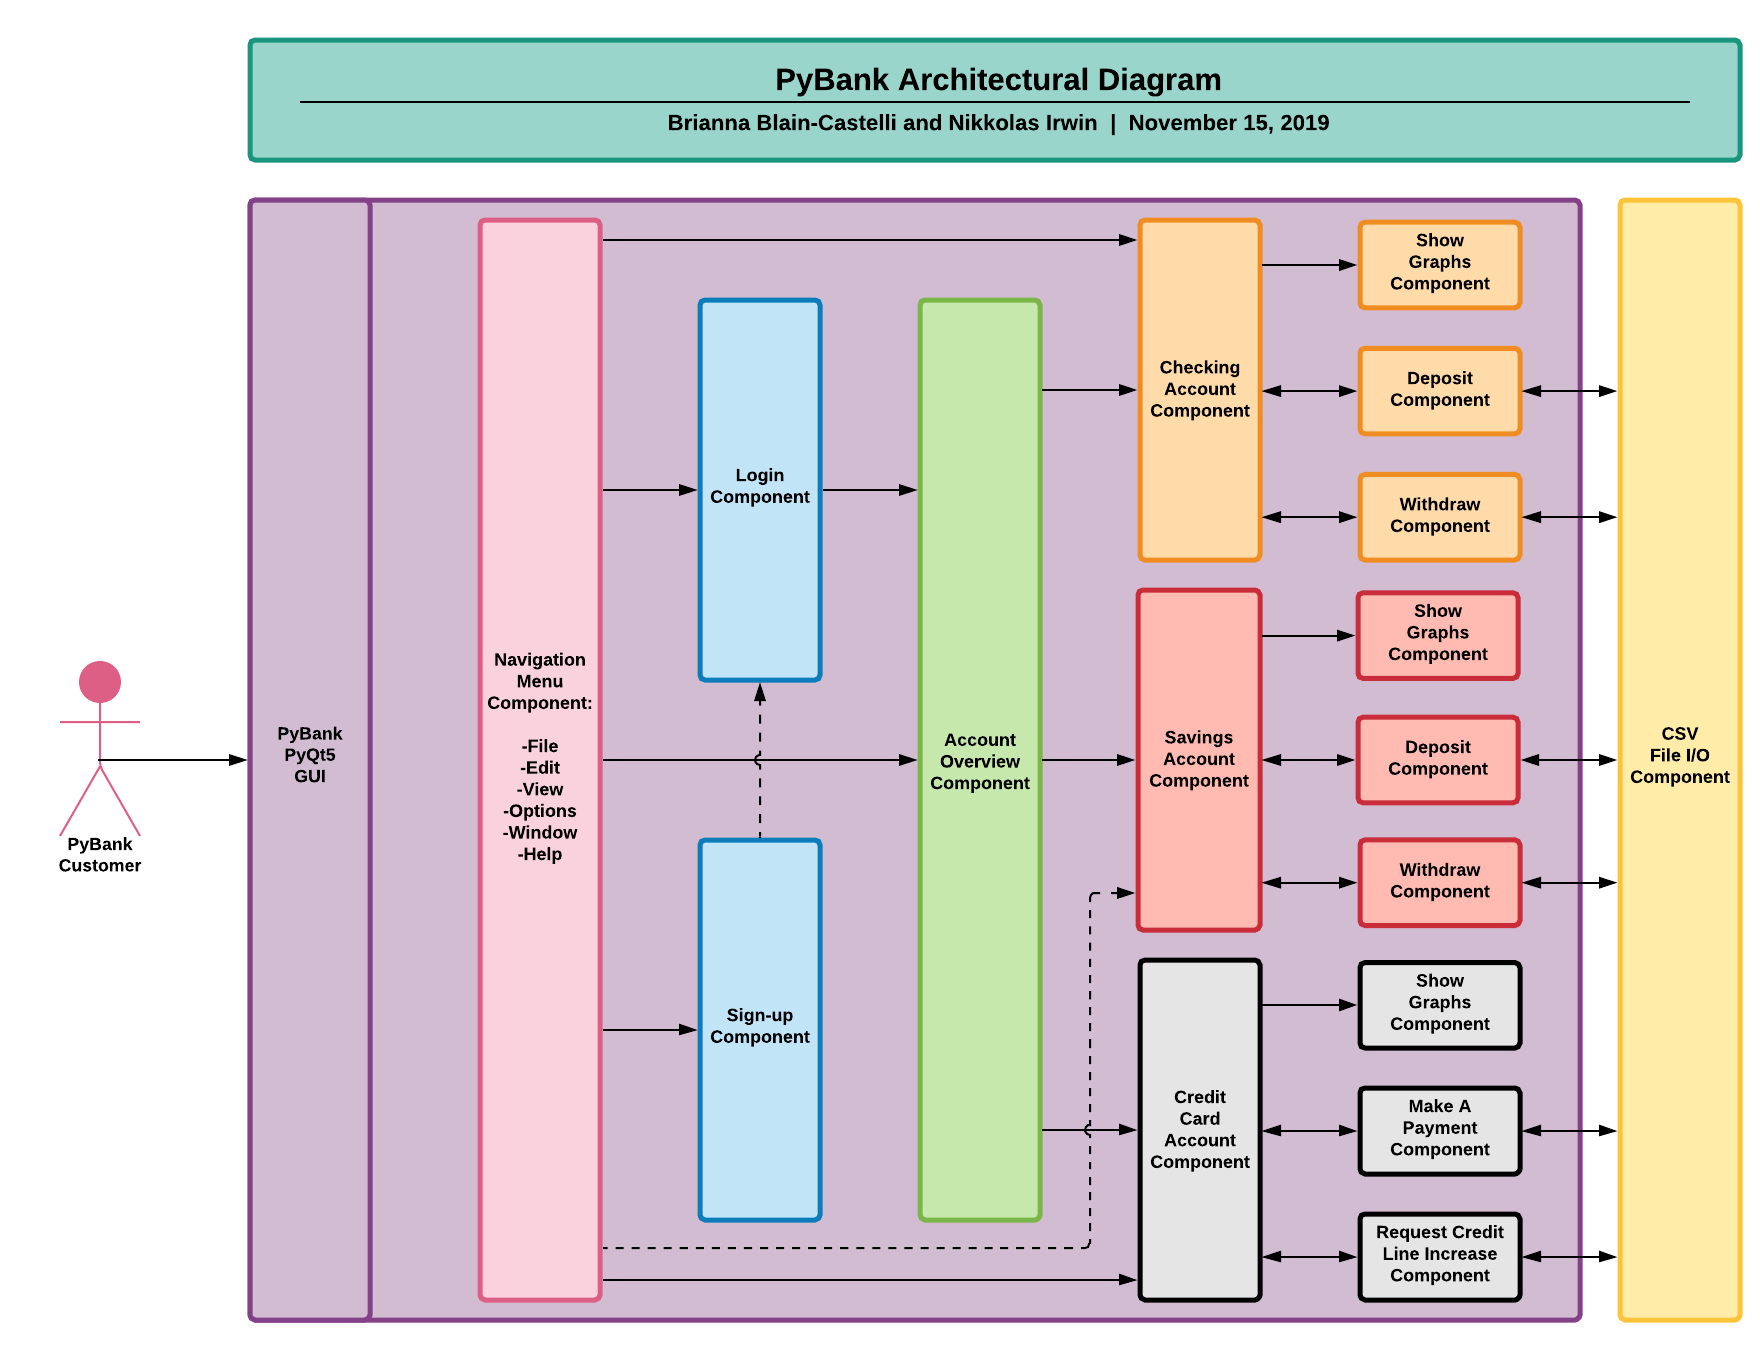
\includegraphics[width=1.00\linewidth, height=0.75\linewidth]{figures/Architectural_Diagram_PyBank.png}
	\caption{An architectural diagram describing the major software components present in PyBank.}
	\label{fig:architectural_diagram}
	\end{centering}
\end{figure}

\newpage

\subsection{System-Level Behavioral Diagram}
\label{sect:activity_diagram}

The activity diagram shown below in Figure~\ref{fig:activity_diagram} depicts the sequence of actions that a PyBank customer would take to either login to their existing account or sign-up for a new account and then log into that account. The activity begins with a PyBank customer executing the desktop client and completes once the PyBank customer has logged into their account and is presented with the \textbf{\textit{Account Overview}} window.

\begin{figure}[H]
	\begin{centering}
	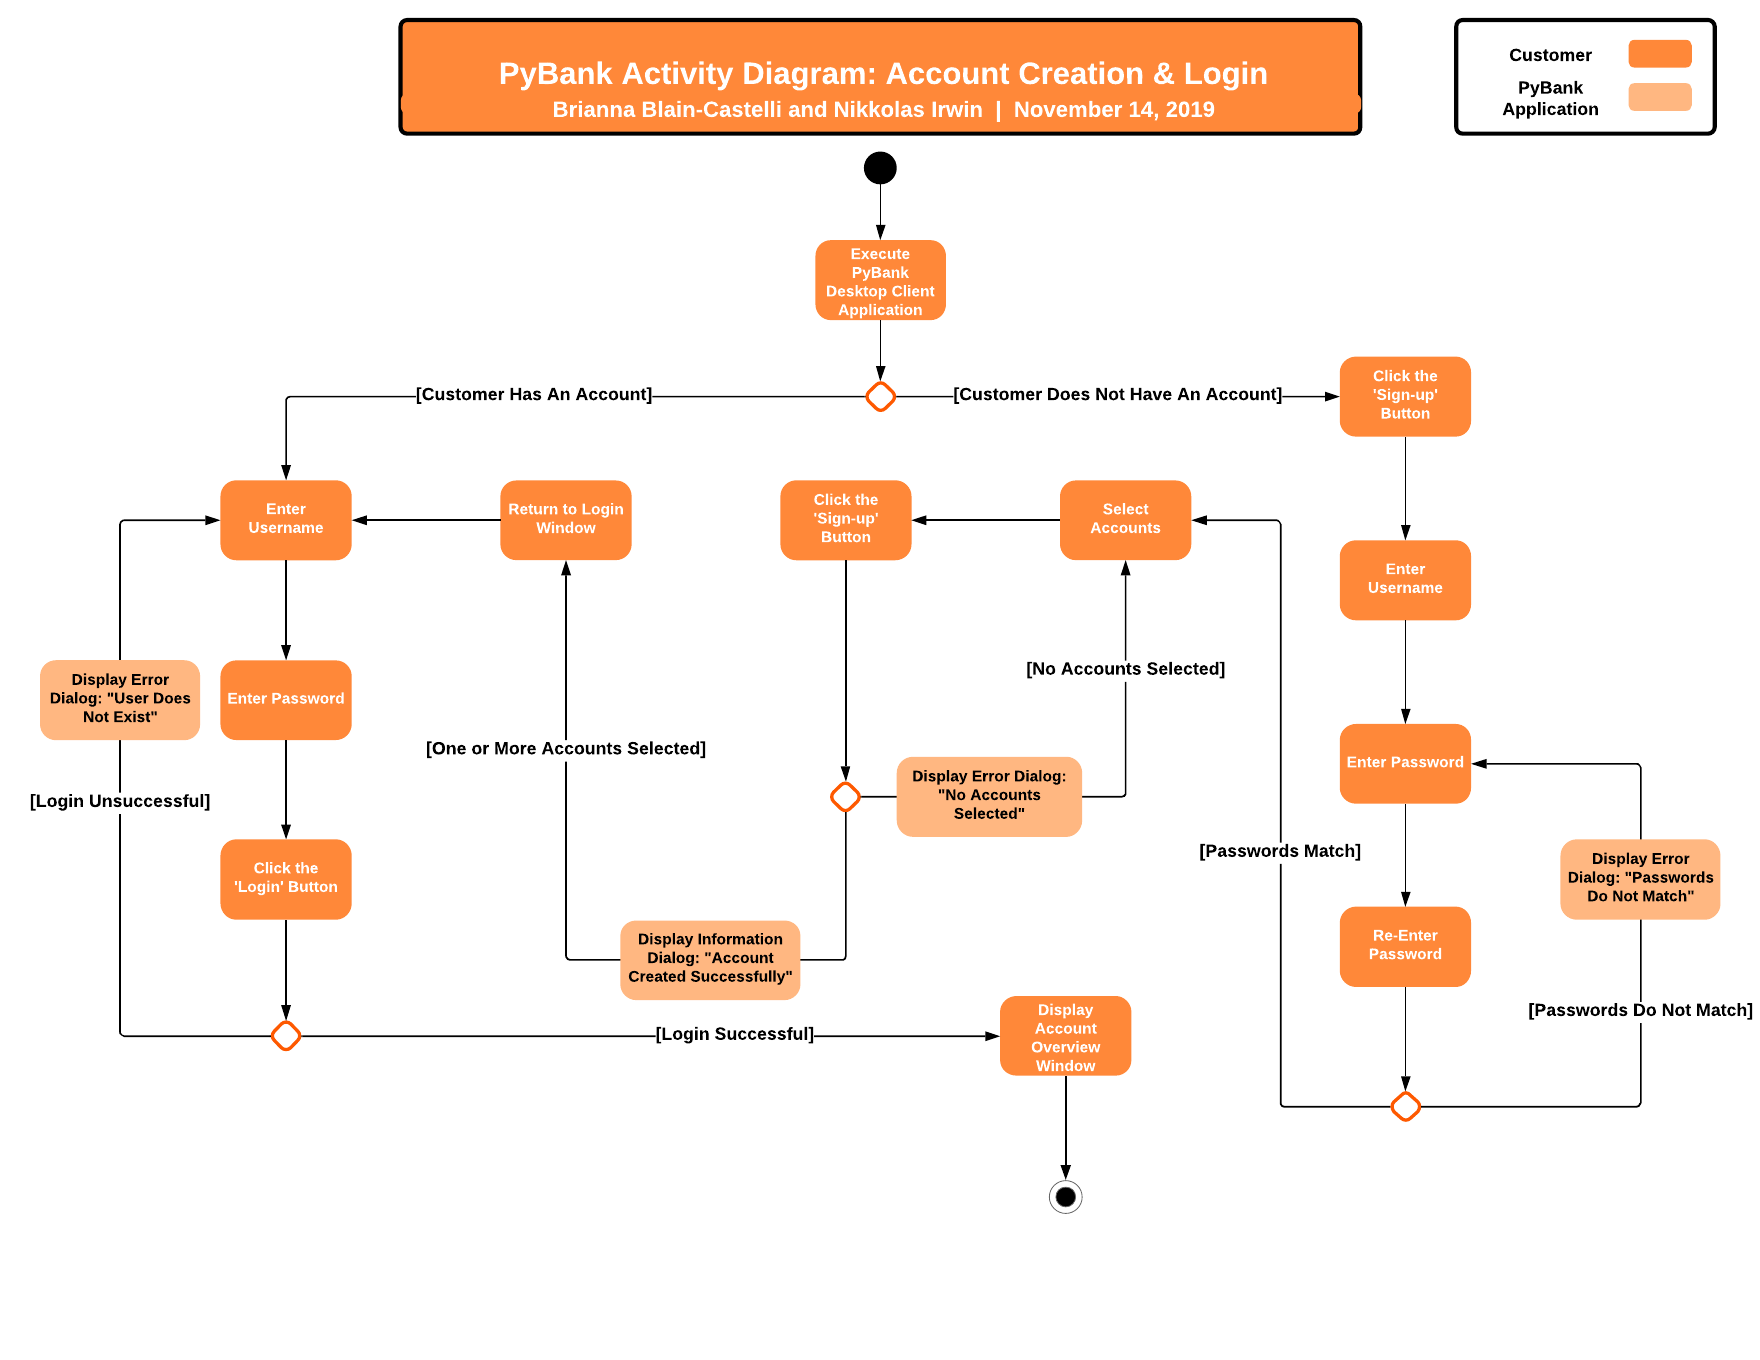
\includegraphics[width=1.00\linewidth, height=0.75\linewidth]{figures/Activity_Diagram_PyBank.png}
	\caption{An activity diagram describing the login and account creation processes in PyBank.}
	\label{fig:activity_diagram}
	\end{centering}
\end{figure}

%EOF
%-----------------------------------END-----OF-----SECTION----------------------------------%
\newpage
%-----------------------------------START-----OF-----SECTION--------------------------------%
\section{Static Interface Design}
\label{sect:static_interface_design}

Mock-ups of key views were created using Balsamiq~\cite{BALSAMIQ_MOCKUPS_3:1}~to illustrate the desired user interface associated with these windows prior to finalized implementation.

\subsection{Sign-in Window}
\label{sect:signin_window}

Figure \ref{fig:signin} shows a mock-up of the login window for PyBank. The icon shown is a current placeholder until a finalized logo for the application can be developed. Password will display a masked version of the entered password for user privacy; however, when holding the eye shaped icon down, the password will show for the user. There is a link to sign-up available, button to sign up, and a button to cancel login and exit the application.

\FloatBarrier
\begin{figure}[!ht]
    \centering
    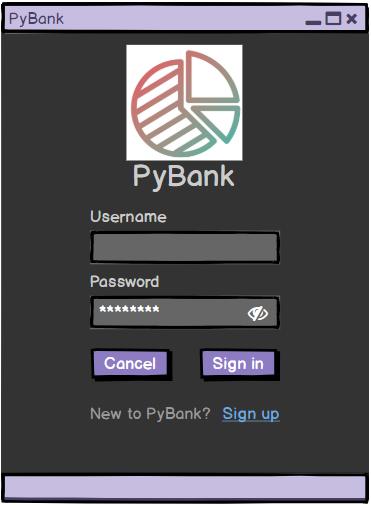
\includegraphics[width=8cm]{figures/signin.png}
    \caption{The Sign-in window for PyBank.}
    \label{fig:signin}
\end{figure}

\newpage

\subsection{Sign-up Window Part II}
\label{sect:signup_window}

Figure \ref{fig:signup} is a mock-up of the second part of the sign-up window. Along the top is a progress bar, showing the user where in the sign-up process they are. Below the progress bar is a title, describing the purpose of the current step in the process. On this window, the user can utilize the checkbox that will grey out all options below besides next and back, keeping the user from entering information and allowing them to skip the window. Otherwise, the user may choose to link a bank account from a partnered bank, or enter account information manually for the user to track finances without linking all information.

\FloatBarrier
\begin{figure}[!ht]
    \centering
    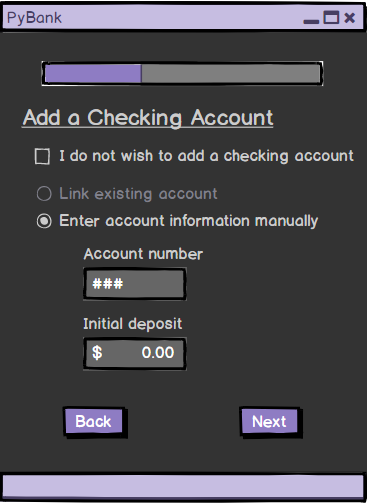
\includegraphics[width=8cm]{figures/signup.png}
    \caption{The Sign-up window part II for PyBank.}
    \label{fig:signup}
\end{figure}

\newpage

\subsection{Account Overview Window}
\label{sect:acct_overview}

Figure \ref{fig:overview} is the account overview. This window provides a brief summary of account information for the user to access at a glance. This includes account balances, account number--which is entered by the user and serves as a form of account identification in the event the user has multiple of the same type of account—and an overview of the most recent transactions. Because this was the most common functionality utilized by stakeholders, it is the first window the user is taken to after signing in.

\FloatBarrier
\begin{figure}[!ht]
    \centering
    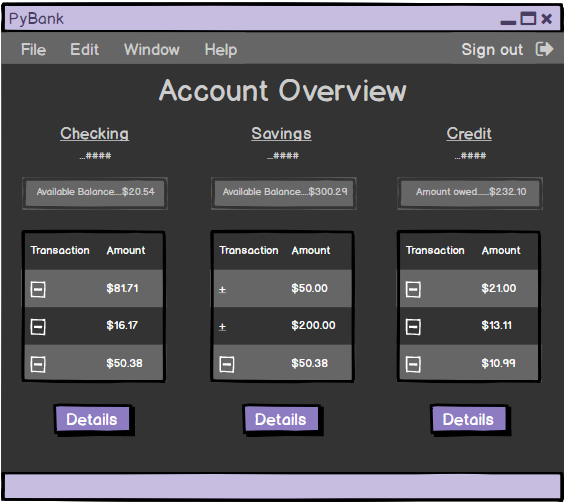
\includegraphics[width=11cm]{figures/accountoverview.png}
    \caption{The account overview window shows basic information relating to all accounts owned by the user.}
    \label{fig:overview}
\end{figure}

\newpage

\subsection{Checking Account Window}
\label{sect:checking_acct}

Figure \ref{fig:details} is the account details window. This window serves to show transaction details, upcoming bills, and a bill calendar. There is a search functionality as well that allows the users to find a specific transaction or bill. Along the top, this window provides options to access graph displays, send money, or transfer money.

\FloatBarrier
\begin{figure}[!ht]
    \centering
    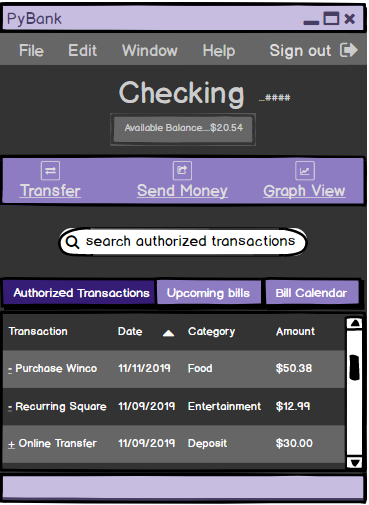
\includegraphics[width=8cm]{figures/accountdetails.png}
    \caption{A detailed view of a specific account's checking account details.}
    \label{fig:details}
\end{figure}

\newpage

\subsection{Online Transfer Funds Window}
\label{sect:online_transfer_funds}

The window for performing online transfers is shown in Figure \ref{fig:transfer}. In this view, the user selects an account from the drop down menu to dictate where money is to be transferred from and where it is to be transferred to. The user then enters a value to transfer between accounts and the date on which the transfer is to take place.

\FloatBarrier
\begin{figure}[!ht]
    \centering
    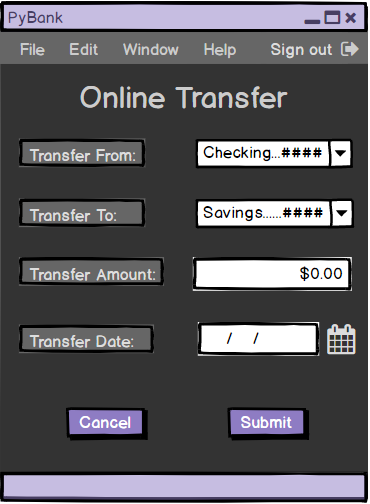
\includegraphics[width=8cm]{figures/transfer.png}
    \caption{A detailed view of a specific account performing an online transfer.}
    \label{fig:transfer}
\end{figure}

\newpage

\subsection{Visualization Window}
\label{sect:visualization_window}

Graphical representations of finances and budgeting are shown in Figure \ref{fig:graphs}. This view allows an alternate was to be able to see summaries of important information to the user. Along the top of the screen is the current graph being displayed. Below that is a set of radio buttons where the user is able to pick from a list of different graphs.

\FloatBarrier
\begin{figure}[!ht]
    \centering
    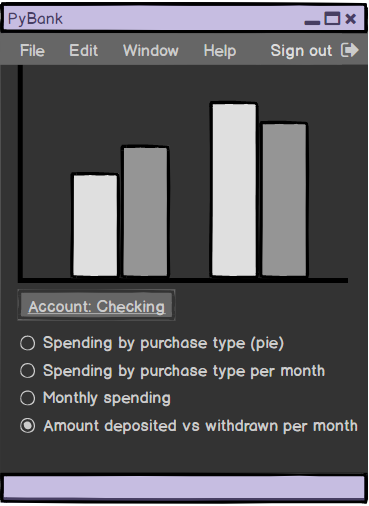
\includegraphics[width=8cm]{figures/accountgraphs.png}
    \caption{A detailed view of a specific account's visualizations.}
    \label{fig:graphs}
\end{figure}

\FloatBarrier
%EOF
%-----------------------------------END-----OF-----SECTION----------------------------------%
\newpage
%-----------------------------------START-----OF-----SECTION--------------------------------%
\section{Alternative Designs}
\label{sect:alternative_designs}

Shown below are two alternative designs that were considered for PyBank but ultimately were discarded for their counterparts which were shown in Section~\ref{sect:static_interface_design}. The first design shown below in Figure~\ref{fig:alt_sign_in_diagram} displays an alternative Sign-in window and the second design also shown below in Figure~\ref{fig:alt_visualization_diagram} displays an alternative checking account visualization window.

\subsection{Alternative Sign-in Window}
\label{sect:alt_sign_in}

The alternative sign-in window displayed below in Figure~\ref{fig:alt_sign_in_diagram} was not chosen for several reasons including the following: the avatar shown in the window should not be placed at the login before the user is known, the window's navigation menu and title do not have a color scheme that helps contrast the bright text colors, and some common window functions (minimizing/maximizing) are also absent from the design. For these reasons, the sign-in window presented in Section~\ref{sect:static_interface_design}, Figure~\ref{fig:signin} was chosen. 

\begin{figure}[H]
	\begin{centering}
	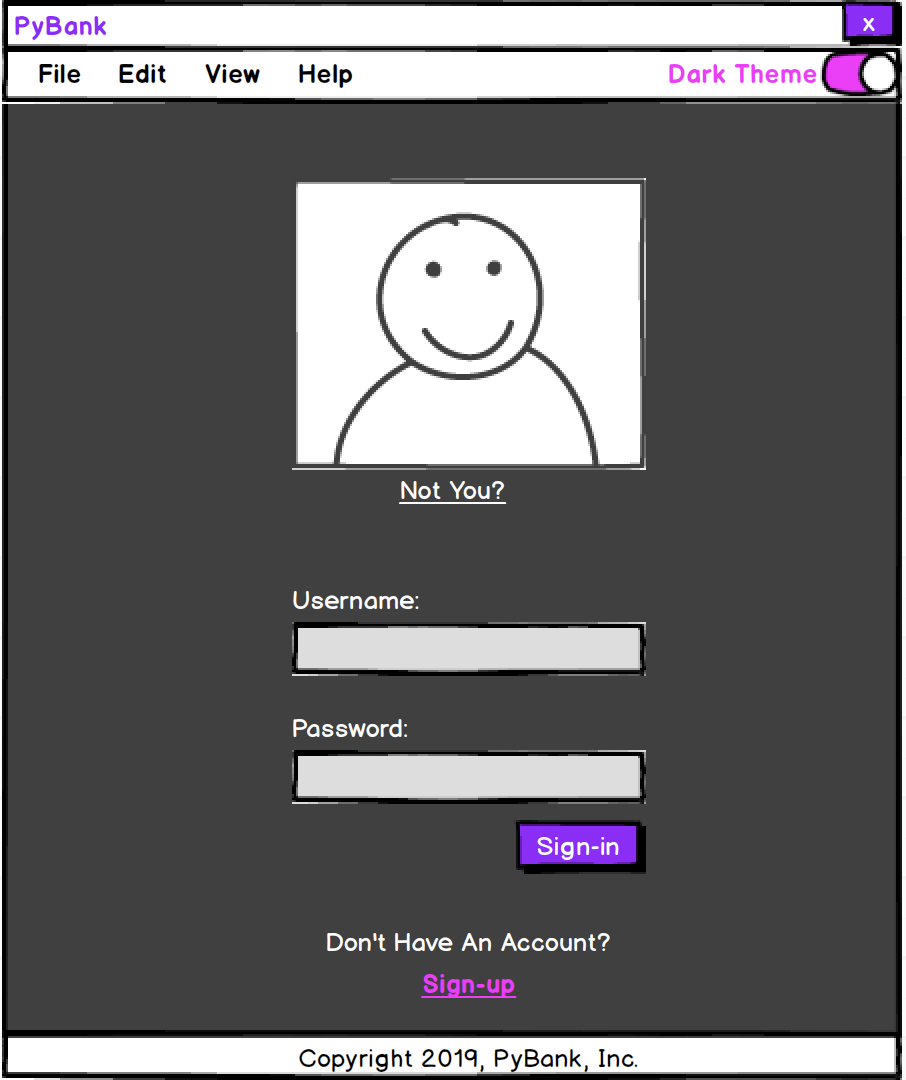
\includegraphics[width=0.55\linewidth, height=0.70\linewidth]{figures/alternative_sign_in_design.png}
	\caption{A medium-fidelity prototype alternative for the sign-in window.}
	\label{fig:alt_sign_in_diagram}
	\end{centering}
\end{figure}

\newpage

\subsection{Alternative Visualization Window}
\label{sect:alt_visualization}

The alternative visualization window for checking accounts shown below in Figure~\ref{fig:alt_visualization_diagram} was not selected for PyBank because it does not provide the user with a wide selection of options. The visualizations presented in the alternative design are limited to \emph{spending vs. time} analysis whereas the chosen design provides radio buttons with multiple criteria that a customer can look at. Other reasons for dismissing this design are similar to the alternative sign-in window where the window's navigation menu and title do not have a color scheme that helps contrast the bright text colors, and some common window functions (minimizing/maximizing) are also absent from the design. For these reasons, the visualization window presented in Section~\ref{sect:static_interface_design}, Figure~\ref{fig:graphs} was chosen.

\begin{figure}[H]
	\begin{centering}
	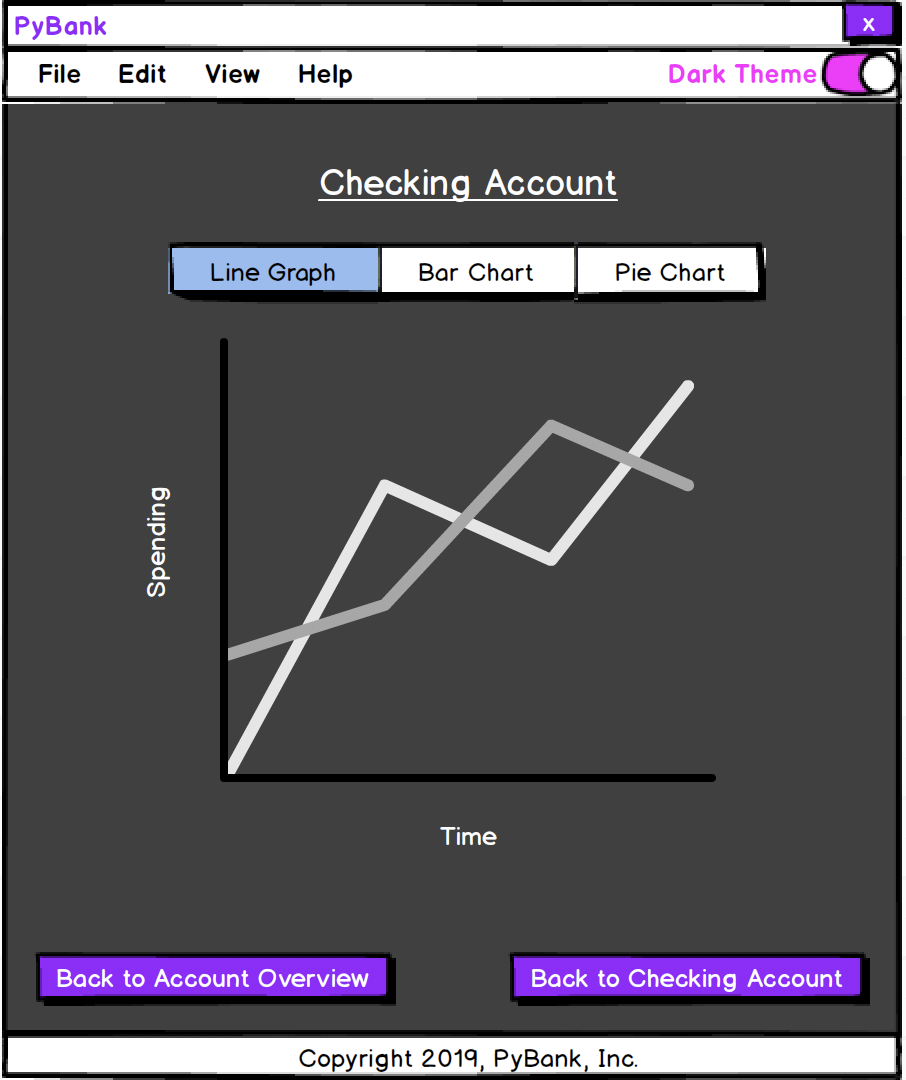
\includegraphics[width=0.55\linewidth, height=0.70\linewidth]{figures/alternative_visualization_design.png}
	\caption{A medium-fidelity prototype alternative for the checking account visualizations window.}
	\label{fig:alt_visualization_diagram}
	\end{centering}
\end{figure}

%EOF
%-----------------------------------END-----OF-----SECTION----------------------------------%
\newpage
%-----------------------------------START-----OF-----SECTION--------------------------------%
\section{Annotated References and Resources}
\label{sect:annotated_references}

Listed below are annotated references which helped produce this document covering PyBank's design. Two of the references, \emph{The Design of Everyday Things}~\cite{THE_DESIGN_OF_EVERYDAY_THINGS:0} and \emph{Designing the User Interface}~\cite{DESIGNING_THE_USER_INTERFACE:6} are utilized by CS 420/620 taught by Dr. Sergiu Dascalu. The other five annotated references helped produce our diagrammatic solutions or have aided with the development of PyBank. All annotated references contain hyperlinks to the \textbf{References}~section which contains the bibliographic information for each reference or resource found at the end of this document.

\subsection{The Design of Everyday Things}
\label{sect:doet}

\emph{The Design of Everyday Things}~\cite{THE_DESIGN_OF_EVERYDAY_THINGS:0} is a book that details good and bad designs in everyday things and presents fundamental properties of good design that are applicable across domains. For PyBank, we've utilized two concepts heavily during our design process. The first concept, \emph{signifiers}, are described by the author Don Norman as ``[...] any mark or sound, any perceivable indicator that communicates appropriate behavior to a person~\cite{THE_DESIGN_OF_EVERYDAY_THINGS:0}." Our design incorporates signifiers through the use of a variety of PyQt5 widgets such as buttons, labels, text boxes, etc. All of these widgets serve to communicate to a PyBank customer the appropriate behavior for an action within the application. We also use another concept presented in the book, \emph{feedback}, to help provide a user with immediate communication related to the results of an action. PyBank accomplishes this feat through the use of error and information dialog boxes.

\subsection{Designing the User Interface}
\label{sect:dtui}

\emph{Designing the User Interface}~\cite{DESIGNING_THE_USER_INTERFACE:6} provides strategies for effective human-computer interaction. This book covers usability, guidelines, principles, theories, the design process, interaction styles, and design issues. One important concept covered in Chapter 4, Section 4.5.5 is prototyping~\cite{DESIGNING_THE_USER_INTERFACE:6}. The book presents three types, low-fidelity, medium-fidelity, and high-fidelity prototypes. Our static interface designs found in Section~\ref{sect:static_interface_design} and our alternative designs found in Section~\ref{sect:alternative_designs} utilized Balsamiq Mockups 3~\cite{BALSAMIQ_MOCKUPS_3:1} which helped us create our medium-fidelity prototypes.

\subsection{Balsamiq Mockups 3}
\label{sect:balsamiq_mockups_3}

\emph{Balsamiq Mockups 3}~\cite{BALSAMIQ_MOCKUPS_3:1} is a software application that provides rapid prototyping through wireframing. One feature of this application are UI Controls such as buttons, text input, drop down menus, radio buttons, menu bars, icons, and many more controls. Another feature of \emph{Balsamiq Mockups 3}~\cite{BALSAMIQ_MOCKUPS_3:1} is the ability to share wireframes with other designers and collaborate across platforms and devices using the technologies like Google Drive, the cloud version of the application, among other things.

\subsection{Lucid Chart}
\label{sect:lucid_chart}

\emph{Lucid Chart}~\cite{LUCID_CHART:2} is a cloud-based diagramming and visualization software solution that is extremely popular. It is endorsed by 99\% of fortune 500 companies and it provides over 500 templates for speeding up the diagramming process. \emph{Lucid Chart}~\cite{LUCID_CHART:2} supports multi-page diagram solutions and allows many designers to collaborate together on the same project. An additional benefit of \emph{Lucid Chart}~\cite{LUCID_CHART:2} is that it supports templates for technologists and business professionals making it a solution for a variety of practitioners.

\subsection{Qt}
\label{sect:qt}

\emph{Qt}~\cite{QT:3} is the official source for documentation for the Qt API. In our case, our work relates specifically to the Python API for Qt. Qt more broadly is a cross-platform software solution for embedded systems and desktop systems. The documentation provided by \emph{Qt}~\cite{QT:3} includes: examples, tutorials, quick-start guides, development tools, and the Qt Creator IDE which supports ``[...] a powerful cross-platform integrated development environment, including UI designer tools and on-device debugging~\cite{QT:3}."

\subsection{ZetCode}
\label{sect:zetcode}

\emph{ZetCode}~\cite{ZETCODE:4} ``[...] brings tutorials for programmers in various areas. The main are Graphical User Interfaces, databases, and programming languages. The website's mission is to provide competent, quick and easy to understand tutorials for modern-day technologies~\cite{ZETCODE:4}." This website is maintained by its author, Jan Bodnar. It has provided useful tutorials for the development of PyBank.

\subsection{Material Design}
\label{sect:material_design}

\emph{Material}~\cite{MATERIAL:7} ``[...] Material is a design system – backed by open-source code – that helps teams build high-quality digital experiences~\cite{MATERIAL:7}." Material provides four main selections from the homepage which are the following: Design, Components, Develop, and Resources. All of these selections have many sub-categories. Material provides a vast set of design tips based on its philosophy for creating user interfaces. Everything from layout to navigation to typography, etc. is covered by the website. Material also provides icons, Google fonts, and many other resources.

%EOF
%-----------------------------------END-----OF-----SECTION----------------------------------%
\newpage
%-----------------------------------START-----OF-----SECTION--------------------------------%
\section{Contributions of Team Members}
\label{sect:contributions}
\subsection{Brianna Blain-Castelli}
\emph{Individual contributions}
\begin{itemize}
    \item {Abstract, Section~\ref{sect:abstract}}
    \item {Static Interface Design, Section~\ref{sect:static_interface_design}}
    \begin{itemize}
        \item {Initial sketches.}
        \item {Mock-up design prototyping utilizing \emph{Balsamiq Mockups 3}~\cite{BALSAMIQ_MOCKUPS_3:1}.}
            \begin{itemize}
                \item {Created and wrote the description for the sign-in window shown in Figure~\ref{fig:signin} using \emph{Balsamiq Mockups 3}~\cite{BALSAMIQ_MOCKUPS_3:1}.}
                \item {Created and wrote the description for the sign-up window part II shown in Figure~\ref{fig:signin} using \emph{Balsamiq Mockups 3}~\cite{BALSAMIQ_MOCKUPS_3:1}.}
                \item {Created and wrote the description for the account overview window shown in Figure~\ref{fig:overview} using \emph{Balsamiq Mockups 3}~\cite{BALSAMIQ_MOCKUPS_3:1}.}
                \item {Created and wrote the description for the checking account window shown in Figure~\ref{fig:details} using \emph{Balsamiq Mockups 3}~\cite{BALSAMIQ_MOCKUPS_3:1}.}
                \item {Created and wrote the description for the online transfer funds window shown in Figure~\ref{fig:transfer} using \emph{Balsamiq Mockups 3}~\cite{BALSAMIQ_MOCKUPS_3:1}.}
                \item {Created and wrote the description for the visualization window shown in Figure~\ref{fig:graphs} using \emph{Balsamiq Mockups 3}~\cite{BALSAMIQ_MOCKUPS_3:1}.}
            \end{itemize}
        \item {Section write-up and captioning.}
        \end{itemize}
\end{itemize}
\subsection{Nikkolas Irwin}
\emph{Individual contributions}
\begin{itemize}
    \item {High-Level Design, Section~\ref{sect:high_level_design}}
        \begin{itemize}
            \item {Created the architectural diagram shown in Figure~\ref{fig:architectural_diagram} using Lucidchart~\cite{LUCID_CHART:2} and provided the written description of the architectural diagram.}
            \item {Created the activity diagram shown in Figure~\ref{fig:activity_diagram}  using Lucidchart~\cite{LUCID_CHART:2} and provided the written description of the activity diagram.}
        \end{itemize}{}
    \item {Alternative Designs, Section~\ref{sect:alternative_designs}}
        \begin{itemize}
            % alt. design 1
            \item {Created and wrote the description for the alternative sign-in window shown in Figure~\ref{fig:alt_sign_in_diagram} using \emph{Balsamiq Mockups 3}~\cite{BALSAMIQ_MOCKUPS_3:1}.}
            % alt. design 2
            \item {Created and wrote the description for the alternative checking account visualization window shown in Figure~\ref{fig:alt_visualization_diagram} using \emph{Balsamiq Mockups 3}~\cite{BALSAMIQ_MOCKUPS_3:1}.}
        \end{itemize}
    \item {Annotated References and Resources, Section~\ref{sect:annotated_references}}
        \begin{itemize}
            % ref. 1
            \item {Wrote the annotated reference for \emph{The Design of Everyday Things}~\cite{THE_DESIGN_OF_EVERYDAY_THINGS:0}, Section~\ref{sect:doet}.}
            % ref. 2
            \item {Wrote the annotated reference for \emph{Designing the User Interface}~\cite{DESIGNING_THE_USER_INTERFACE:6}, Section~\ref{sect:dtui}.}
            % ref. 3
            \item {Wrote the annotated reference for \emph{Balsamiq Mockups 3}~\cite{BALSAMIQ_MOCKUPS_3:1}, Section~\ref{sect:balsamiq_mockups_3}.}
            % ref. 4
            \item {Wrote the annotated reference for \emph{Lucid Chart}~\cite{LUCID_CHART:2}, Section~\ref{sect:lucid_chart}.}
            % ref. 5
            \item {Wrote the annotated reference for \emph{Qt}~\cite{QT:3}, Section~\ref{sect:qt}.}
            % ref. 6
            \item {Wrote the annotated reference for \emph{ZetCode}~\cite{ZETCODE:4}, Section~\ref{sect:zetcode}.}
            % ref. 7
            \item {Wrote the annotated reference for \emph{Material}~\cite{MATERIAL:7}, Section~\ref{sect:material_design}.}
        \end{itemize}
\end{itemize}
%EOF
%-----------------------------------END-----OF-----SECTION----------------------------------%
\newpage
%-----------------------------------START-----OF-----SECTION--------------------------------%
\phantomsection
\addcontentsline{toc}{section}{References}
\label{sect:references}
\bibliography{main.bib}
\bibliographystyle{ieeetr}

% EOF
%-----------------------------------END-----OF-----SECTION----------------------------------%

\end{document}
